\documentclass{article}
\usepackage[italian]{babel}
\usepackage[tmargin=2cm,rmargin=1.5in,lmargin=1.5in,margin=0.85in,bmargin=2cm,footskip=.2in]{geometry}
\usepackage{siunitx}
\sisetup{separate-uncertainty=true, per-mode=fraction, parse-numbers=true}
\usepackage{caption}
\usepackage[T1]{fontenc}
\usepackage{bookmark}
\usepackage{mathcomp}
\usepackage{graphicx}
\usepackage{multicol}
\usepackage{booktabs}
\usepackage{amsmath,amsfonts,amsthm,amssymb,mathtools}
\hypersetup{
	pdftitle={Relazione sul pendolo quadrifilare},
	colorlinks=true, linkcolor=doc!90,
	bookmarksnumbered=true,
	bookmarksopen=true
}
\usepackage{blindtext}
\usepackage{wrapfig}
\usepackage{listings}
\usepackage{xcolor}
\usepackage{float}
\usepackage{tikz}
\usepackage{multirow}
\usepackage{biblatex}
\definecolor{codegreen}{rgb}{0,0.6,0}
\definecolor{codegray}{rgb}{0.5,0.5,0.5}
\definecolor{codepurple}{rgb}{0.58,0,0.82}
\definecolor{backcolour}{rgb}{0.95,0.95,0.92}
\definecolor{doc}{rgb}{0,0,0}
\lstdefinestyle{code}{
    backgroundcolor=\color{backcolour},   
    commentstyle=\color{codegreen},
    keywordstyle=\color{magenta},
    numberstyle=\tiny\color{codegray},
    stringstyle=\color{codepurple},
    basicstyle=\ttfamily\footnotesize,
    breakatwhitespace=false,         
    breaklines=true,                 
    captionpos=b,                    
    keepspaces=true,                                     
    showspaces=false,                
    showstringspaces=false,
    showtabs=false,                  
    tabsize=2,
    inputencoding=ansinew,
    extendedchars=true,
    numbers=left,                    
    numbersep=5pt
}

\lstset{style=code}
\usepackage[varbb]{newpxmath}
\usepackage{circuitikz}
\captionsetup{labelfont={bf, sc}}
\title{Relazione sul pendolo quadrifilare}
\author{Aiello Giosuè, Fenili Domenico, Sermi Francesco}
\date{\today}
\begin{document}
	\maketitle
	\newpage
	\tableofcontents
	\newpage
	\section{Scopo}
		Stabilire la dipendenza che sussiste fra il periodo dell'oscillazione e la sua ampiezza
	\section{Cenni teorici}
	Il pendolo fisico (o il pendolo semplice, che può essere visto come caso particolare del pendolo fisico) può essere schematizzato come un corpo rigido soggetto ad una forza peso che induce un momento torcente rispetto al perno $O$ e la reazione vincolare $R$ (che non induce un momento torcente rispetto al polo $O$) che agiscono sulla massa $m$, da cui si ricava utilizzando la $2^a$ cardinale:
	\begin{equation}
		\frac{d\vec{L}}{dt} = I\ddot{\theta} = -mgl\sin{\theta}
	\end{equation}
	che è un problema di Cauchy ben definito
	\begin{align}
		\begin{cases*}
			\ddot{\theta} = - \frac{mgL}{I} \sin{\theta} \\
			\theta(0) = \theta_0 \\
			\dot{\theta}(0) = 0
		\end{cases*}
	\end{align}
	da cui, utilizzando l'ipotesi delle piccole oscillazioni e considerando l'espansione in serie di Taylor della funzione $\sin{(x)} = \sum\limits_{n=0}^{+\infty} \frac{(-1)^n}{(2n+1)!} x^{2n+1}$, possiamo ricondurlo all'equazione di un oscillatore armonico:
	\begin{equation}
		I\ddot{\theta} = -mgl\theta \implies \ddot\theta = -\frac{mgL}{I}\theta
	\end{equation}
	Da cui si ricava che, ponendo $-\omega^2 = -\frac{mgL}{I}$, che il periodo di oscillazione è pari a
	\begin{equation}
		T = 2\pi \sqrt{\frac{I}{mgL}}
	\end{equation}
	da cui si vede che il periodo di oscillazione non dipende, nell'ipotesi delle piccole oscillazioni, dall'angolo di oscillazione iniziale $\theta_0$. \\	
	Se non ipotizziamo le piccole oscillazioni, si può dimostrare che, partendo dal problema di Cauchy di prima
	\begin{align*}
		\ddot{\theta} \cdot 2 \dot{\theta} = -2\frac{mgL}{I}\dot{\theta}\sin{\theta} \implies \int_0^T \frac{d\dot{\theta}^2}{dt} dt = \int_0^T -2\frac{mgL}{I}\dot{\theta}\sin{\theta} dt \implies \dot{\theta}^2 = \frac{2mgL}{I}(\cos{\theta} - \cos{\theta_0})
	\end{align*}
	da cui possiamo 
	\begin{align*}
		&\dot{\theta} = \pm \sqrt{\frac{2mgL}{I}(\cos{\theta} - \cos{\theta_0})} \implies \pm \frac{d\theta}{\sqrt{\frac{2mgL}{I}(\cos{\theta} - \cos{\theta_0})} } = dt
	\end{align*}
	e, integrando e sfruttando l'espansione in serie del coseno\footnote{oppure tramite il fatto che $\cos{x} = \cos{2\frac{x}{2}} = 1 - \sin^2{\frac{x}{2}}$ e con una serie di sostituzione, è possibile ricondursi ad un integrale ellittico completo di prima specie}, è possibile dimostrare che
	\begin{equation}
		T = T_0 \left( 1 + \frac{1}{16}\theta_0^2 + \frac{11}{3072}\theta_0^4 + \cdots \right)
	\end{equation}
	dove $T_0 = 2\pi\sqrt{\frac{l}{g}}$
	Ragionando in termini energetici, si osserva che l'energia meccanica si conserva nel moto (supponendo che non ci siano attriti) del pendolo e si ha che

\begin{table}[H]
    \centering
    \begin{tabular}{l c}
        $E_0 = mgl(1-\cos{\theta})$ & \multirow{2}{*}{$\implies \theta_0 = \arccos{ \left(1 - \frac{v_0^2}{2gL} \right)}$} \\
         $E_0 = \frac{1}{2}mv_0^2$ &  \\
    \end{tabular}
\end{table}

\noindent Dunque per calcolare l'angolo $\theta_0$ da cui è partito il pendolo possiamo utilizzare la velocità $v_0$ con cui arriva sulla verticale del pendolo con la seguente formula:
\begin{equation}
	\theta_0 = \arccos{\left(1- \frac{v_0^2}{2gL} \right) }
	\label{angolo}
\end{equation}
	\section{Strumenti e materiali}
	\textbf{Materiali}:
	\begin{itemize}
		\item Pendolo quadrifilare;
	\end{itemize}
	\textbf{Strumenti}:
	\begin{itemize}
		\item Computer con programma di acquisizione;
		\item Metro a nastro, con sensibilità pari a $\pm 0.001 \, \si{m}$;
		\item Calibro ventesimale, con sensibilità pari a $\pm 0.005 \, \si{\centi\meter}$;
		\item Fotocellula;
	\end{itemize}
	\section{Descrizione delle misure}
	Per effettuare questo esperimento era necessario misurare la velocità del pendolo quando incontrava la verticale, ovvero quando $\theta = 0$ e il periodo di oscillazione del pendolo. 
	\begin{figure}[htbp]
		\centering
  		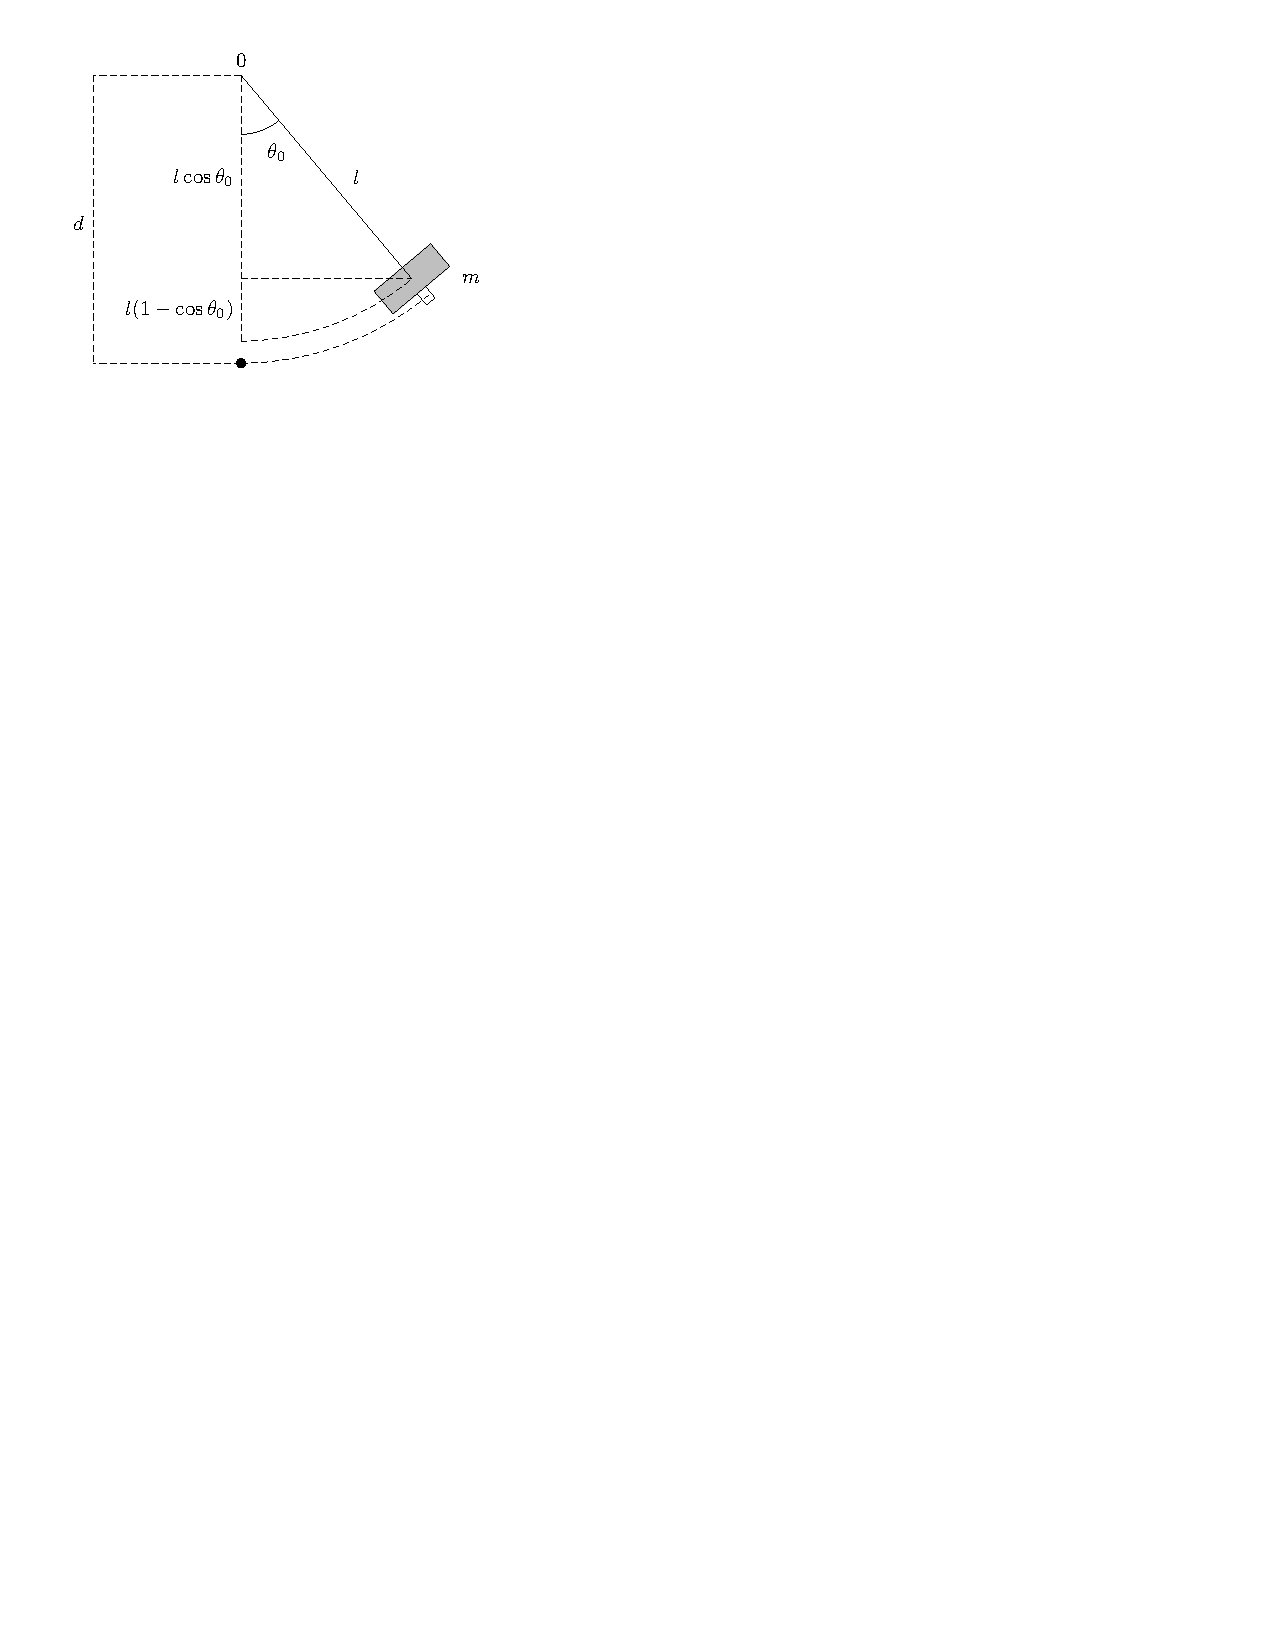
\includegraphics[scale=0.80]{pendolo_fisico_2.pdf}
  		\caption{Schematizzazione del nostro apparato sperimentale: il pendolo, nel laboratorio, è in realtà sorretto da 4 fili che agiscono, complessivamente, come un unico filo di massa trascurabile e di lunghezza $L$ che collega il perno al CM del corpo. La massa $m$ presenta, inoltre, una sbarretta di ferro a distanza $d$ che utilizziamo per coprire una fotocellula che ci misura l'istante in cui la fotocellula viene coperta, il periodo dell'oscillazione del pendolo con la velocità che possiede passando la verticale e il tempo transiente, ovvero il tempo in cui la sbarretta copre completamente la fotocellula. Da notare che la sbarretta, trovandosi a distanza $d$, viaggia ad una velocità maggiore rispetto al centro di massa}
  		\label{fig:pendolo}
	\end{figure}	
	Per fare ciò ci siamo serviti di una fotocellula e di un programma di acquisizione che misurava ogni istante in cui il corpo attivava la fotocellula, il periodo dell'oscillazione che il pendolo stava compiendo (siccome gli attriti dell'aria non sono trascurabili) e il \emph{tempo transiente}, ovvero il tempo in cui il nostro pendolo quadrifilare andava ad oscurare con la sbarretta la fotocellula. Per calcolare tutte le grandezze necessarie per l'esperienza, abbiamo misurato la lunghezza $L$, ovvero la lunghezza del CM del corpo dal perno di rotazione, la lunghezza $d$, ovvero la distanza del perno dal punto della sbarretta che verticalmente oscurava la fotocellula, e la larghezza $w$ della sbarretta; che risultano essere pari a
\begin{align*}
	&L = (1.150 \pm 0.001) \, \si{\meter} & &d = (1.180 \pm 0.001) \, \si{\meter} & &w = (2.050 \pm 0.005) \, \si{\centi\meter}
\end{align*}
Tramite il tempo transiente $\tau$ e la larghezza $w$ era possibile calcolare la velocità media della sbarretta nel punto a distanza $d$ quando passava per la verticale, approssimando il piccolo arco che il pendolo percorreva alla distanza $w$ misurata. 

\begin{table}[H]
\centering
\begin{tabular}{c c c}
Istante di tempo $t_i$ & Periodo dell'oscillazione $T_i$ & Tempo transiente $\tau_i$ \\ 
$(s)$ & $(s)$ & $(s)$ \\ \toprule
2.213801	 & 2.132373 & 0.033546 \\
3.279993	 & 2.132355 & 0.033610 \\
4.346156 & 2.132335	& 0.033688 \\
5.412328	 & 2.132311	& 0.033756 \\
6.478467	 & 2.132285	& 0.033818 \\
7.544613	 & 2.132260	& 0.033886 \\ \bottomrule
\end{tabular}
\caption{Esempi di misurazione effettuato dal programma. Nella prima tabella è riportato l'istante di tempo $t_i$ in cui la sbarretta di ferro montata sulla massa $m$ oscurava la fotocellula, il periodo di oscillazione $T_i$ stimato dal programma di acquisizione che la massa $m$ possedeva con la velocità $v_0$ e il tempo transiente $\tau_i$, ovvero il tempo in cui la sbarretta di ferro copriva la fotocellula}
\end{table}

\noindent Tuttavia noi eravamo interessati a calcolare la velocità del centro di massa che è possibile calcolare con la seguente formula (che si può ricavare tramite le coordinate polari e supponendo che, nell'intervallo di tempo \emph{piccolo}, rispetto alle altre grandezze in gioco, in cui passa per la fotocellula, la velocità angolare sia costante)
\begin{equation}
	v_{CM} = \frac{w}{\tau}\frac{l}{d}
\end{equation}
a cui possiamo assegnare l'incertezza tramite la seguente formula
\begin{equation}
	\sigma_{v_{CM}} = v_{CM} \sqrt{ \left( \frac{\sigma_w}{w} \right)^2 + \left( \frac{\sigma_{\tau_i}}{\tau_i} \right)^2 + \left( \frac{\sigma_l}{l} \right)^2 + \left( \frac{\sigma_d}{d} \right)^2}
\end{equation}
Tuttavia che errore possiamo assegnare a $\tau_i$? Considerando che la misura del \emph{tempo transiente} viene fatta da uno strumento digitale allora tutti i valori compresi nel range della sensibilità dello strumento sono equiprobabili, dunque l'errore che possiamo assegnare a $\tau_i$ è pari a
$$
	\sigma_{\tau_i} = \frac{4}{\sqrt{12}} \, \si{\micro\second}
$$
Abbiamo prima effettuato il grafico del periodo in funzione del tempo, da cui ci si aspettava che il periodo $T$ diminuisse nel corso del tempo (siccome agiscono gli attriti dell'aria)
\begin{figure}[H]
	\centering
	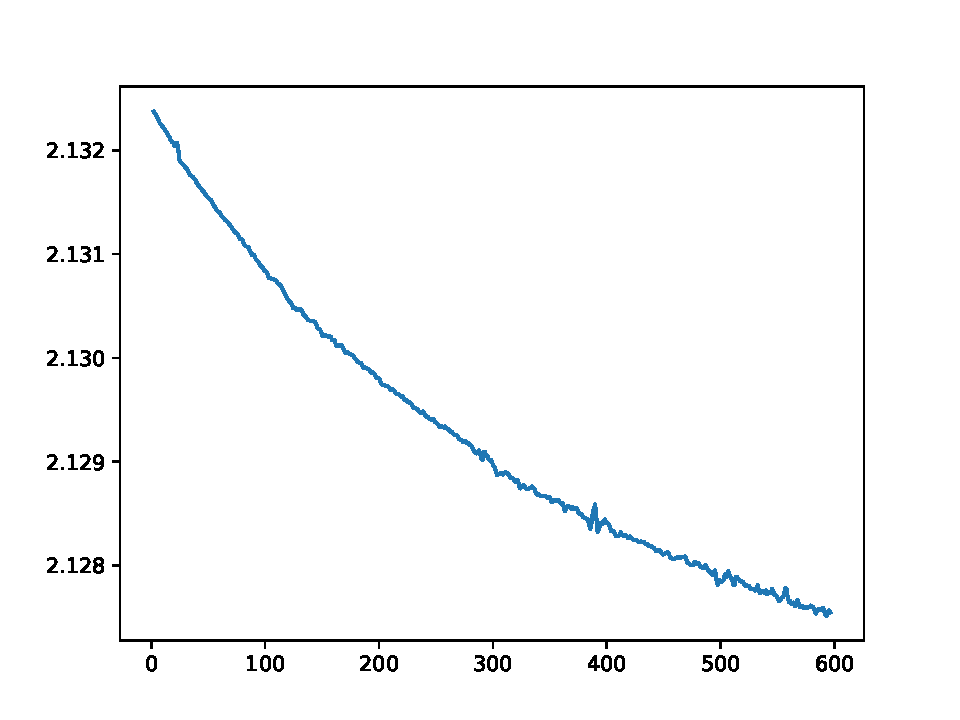
\includegraphics[scale=0.45]{Grafico_periodo_tempo.pdf}
	\caption{Grafico del periodo in funzione del tempo: si osserva che il periodo, come atteso teoricamente, diminuisce nel corso del tempo. Le \emph{spezzate} che si osservano nel grafico possono derivare da \emph{colpi} che sono stati dati inavvertitamente al banco e, siccome il pendolo era molto sensibile, si sono fatte \emph{sentire} }
\end{figure}
A quel punto, abbiamo voluto utilizzare il metodo del fit tramite parametri liberi del grafico velocità-tempo che, a causa dello smorzamento dovuto alle forze di attrito (supponendo che la forza di attrito agisca proporzionalmente alla velocità del centro di massa), deve risultare essere della forma
\begin{equation}
	v_{CM} (t) = v_{CM} (0) e^{-\lambda t}
\end{equation}
dove $v_{CM}(0)$ rappresenta la velocità posseduta dal centro di massa quando oscura la fotocellula la prima volta.
\\

\begin{wrapfigure}{l}{0.50\textwidth}
	\vspace{-1cm}
	\centering
	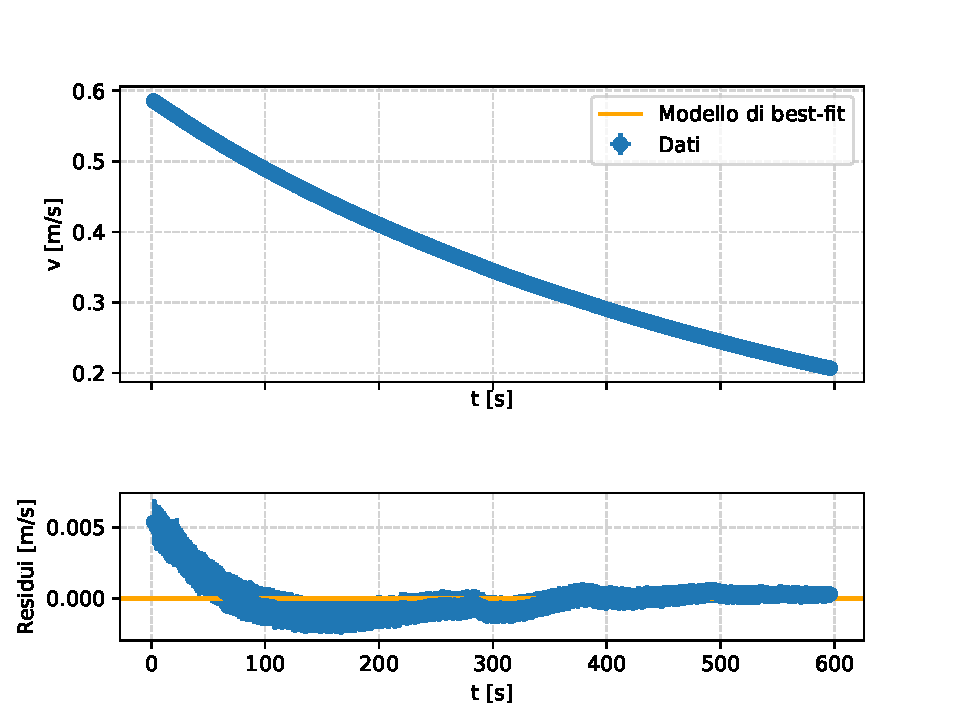
\includegraphics[scale=0.80, width=0.5\textwidth]{Fit_velocita.pdf}
	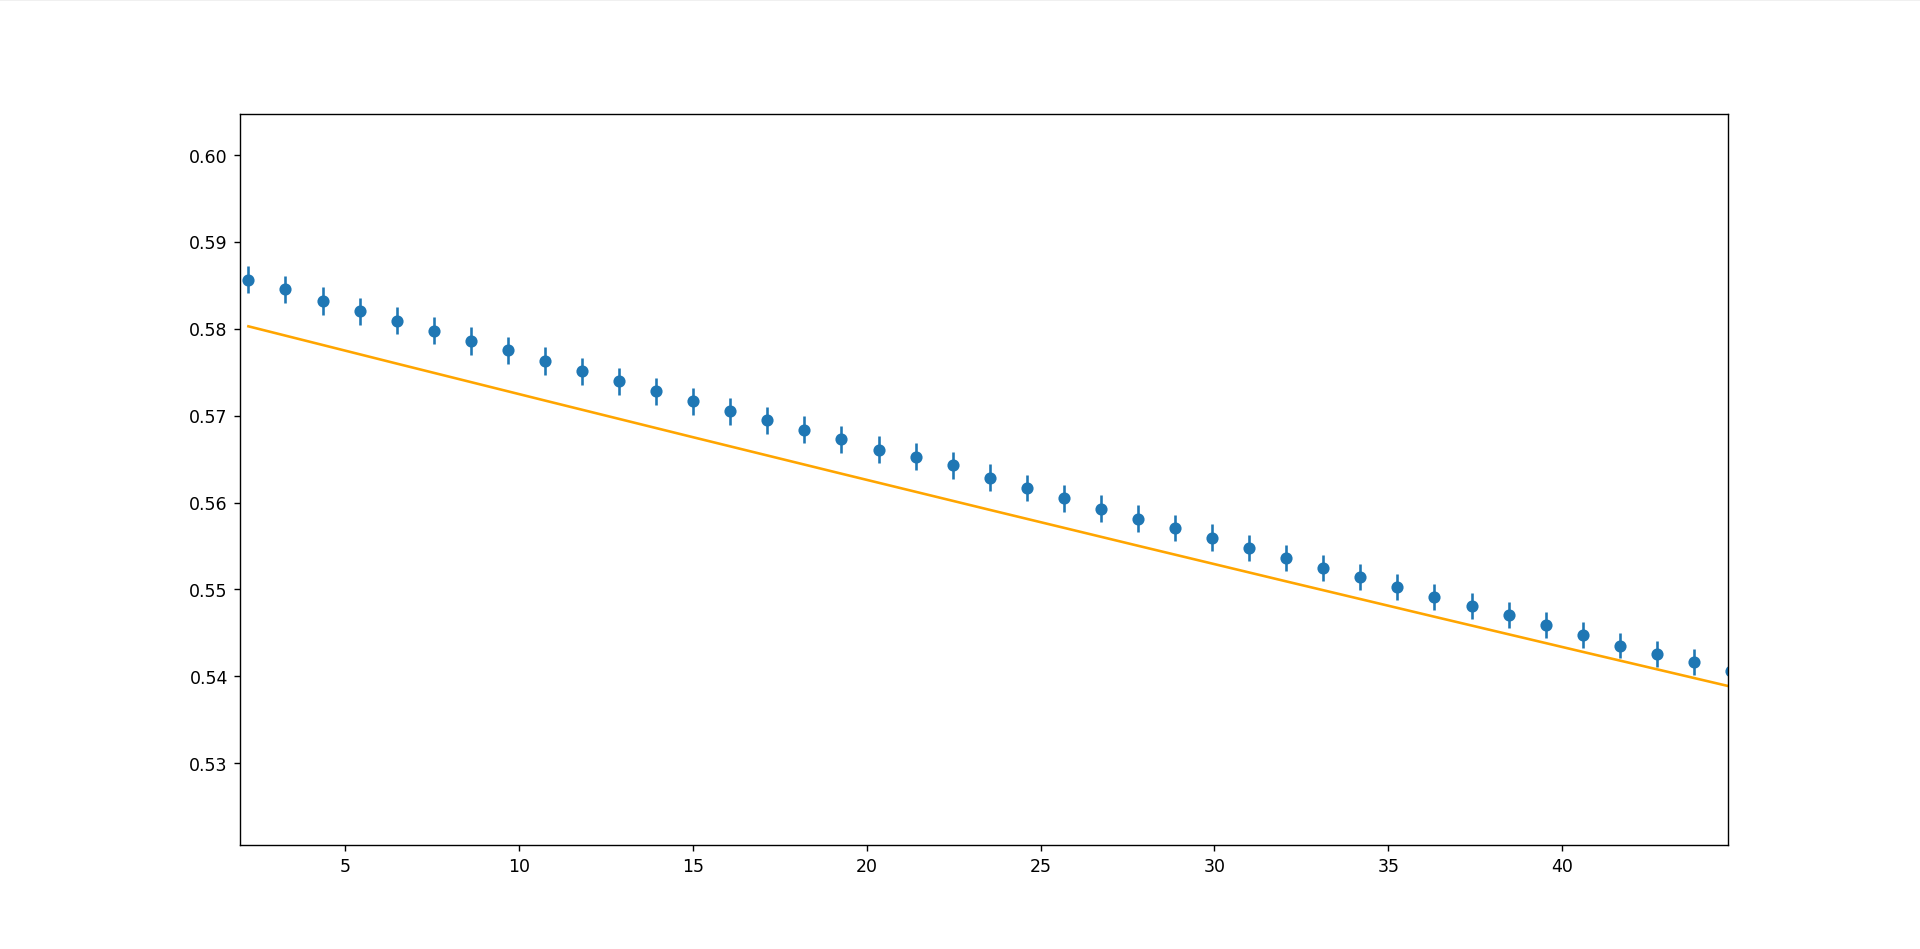
\includegraphics[scale=0.40, width=0.5\textwidth, height=6cm]{pendolo_quadrifilare_zoom.png}
	\caption{Fit del modello teorico con $v_0$ e $\lambda$ come parametri di liberi, zoom di una porzione del fit e grafico dei residui: si osserva che, guardando esclusivamente il fit, questo risulta essere \emph{buono} siccome, a parte per i primi (visibili nello zoom che ho effettuato), i punti sono compatibili, entro le barre di errore, con il fit. Dal grafico dei residui, a parte per i primi (come avevamo già dedotto dal grafico del fit) che non sono compatibili entro le barre di errore con l'asse $y=0$, i punti sono tutti compatibili sebbene ci siano numerose permanenze e i punti non oscillano intorno allo zero distribuendosi in maniera per lo più casuale indica che il nostro modello teorico va a sovrastimare il reale valore atteso. Una probabile spiegazione di questo effettuo è forse dovuto al fatto che il nostro modello teorico suppone che l'attrito dell'aria sia uno smorzatore ideale dunque proporzionale alla velocità del centro di massa, ma nella realtà la forza di attrito dipende anche dalla geometria del corpo}
\end{wrapfigure}
\noindent Effettuando l'analisi del $\chi_2$, si osserva che, questo risulta essere circa
$$
	\chi^2 \approx 410
$$
e, in questo caso, abbiamo un numero di gradi di libertà del fit pari a $557$. Sebbene il valore del $\chi_2$ si discosta significativamente dal valore atteso, è comunque abbastanza \emph{ragionevole} siccome stiamo operando con un modello che tiene conto delle forze di attrito come proporzionali alla velocità, ma ne trascura effetti come la forma del corpo che però ne influenzano il moto. \\
I parametri stimati dal fit risultano esseri pari a
\begin{align}
	&v_0 = (0.5825 \pm 0.0001) \, \si{\meter\per\second} \\
	&\lambda = (0.0017382 \pm 0.0000006)\, \si{\second^{-1}}
\end{align}
che risultano essere ragionevoli, siccome il valore di $v_0(0)$ misurato è pari a $(0.586 \pm 0.002) \, \si{\meter\per\second}$ e dunque dista dal valore stimato dal fit per una distanza pari a $1.75\sigma$ che, considerando le dissipazioni dovute all'attrito, è un valore \emph{abbastanza} ragionevole; per quanto riguardo il parametro $\lambda$ si osserva che il tempo di smorzamento $\tau = \frac{1}{\lambda}$ atteso è circa $580 \, \si{\second}$ (siccome si osserva che la velocità si è ridotta di un fattore pari ad $\frac{1}{e}$) dunque, avendo utilizzato $\lambda$, ci dovrebbe aspettare un valore circa pari a $0.0017 \, \si{\second^{-1}}$. \\
A questo punto abbiamo studiato la dipendenza fra il periodo dell'oscillazione e l'angolo $\theta_0$ effettuando il fit di 2 diversi modelli teorici: il primo era l'espansione in serie di Taylor del periodo dell'oscillazione fino all'ordine $n=2$ e il secondo fino all'ordine $n=4$. In formula:
\begin{align}
	&T(\theta) = T_0 \left(1 + \frac{1}{16}\theta_0^2 \right) \\
	&T(\theta) = T_0 \left(1 + \frac{1}{16}\theta_0^2 + \frac{11}{3072}\theta_0^4 \right)
\end{align}
Tuttavia sorge la domanda di quale errore porre al periodo di oscillazione misurato dallo strumento: non sapendo che tipo di operazioni matematiche il programma di acquisizione effettuava per calcolare il periodo che misurava ogni volta in cui la sbarretta di ferro copriva la fotocellula, abbiamo osservato le varie misure e abbiamo osservato che la differenza fra un periodo ed un altro non è mai inferiore a circa $0.0001 \, \si{\second}$ dunque abbiamo deciso di utilizzare questo valore come \clearpage \noindent una sorta di \emph{sensibilità} su ogni misura del periodo. Per quanto riguarda il calcolo di $\theta$, abbiamo utilizzato la formula~\ref{eq:angolo} e abbiamo assegnato un'incertezza pari a
$$
	\sigma_{\theta_0} = \left| {\frac{1}{\sqrt{1-k^2}}\sigma_k} \right|
$$
\noindent dove $k = 1-\frac{v_0^2}{2gL}$ a cui abbiamo assegnato un'incertezza pari a
$$	
	\sigma_k = k \sqrt{ 2 \left(\frac{\sigma_{v_0}}{v_0} \right)^2 + \left(\frac{\sigma_L}{L} \right)^2}
$$
A questo punto non rimaneva altro che fare i grafici $T-\theta$, fittando i due modelli teorici:
\begin{figure}
	\centering
	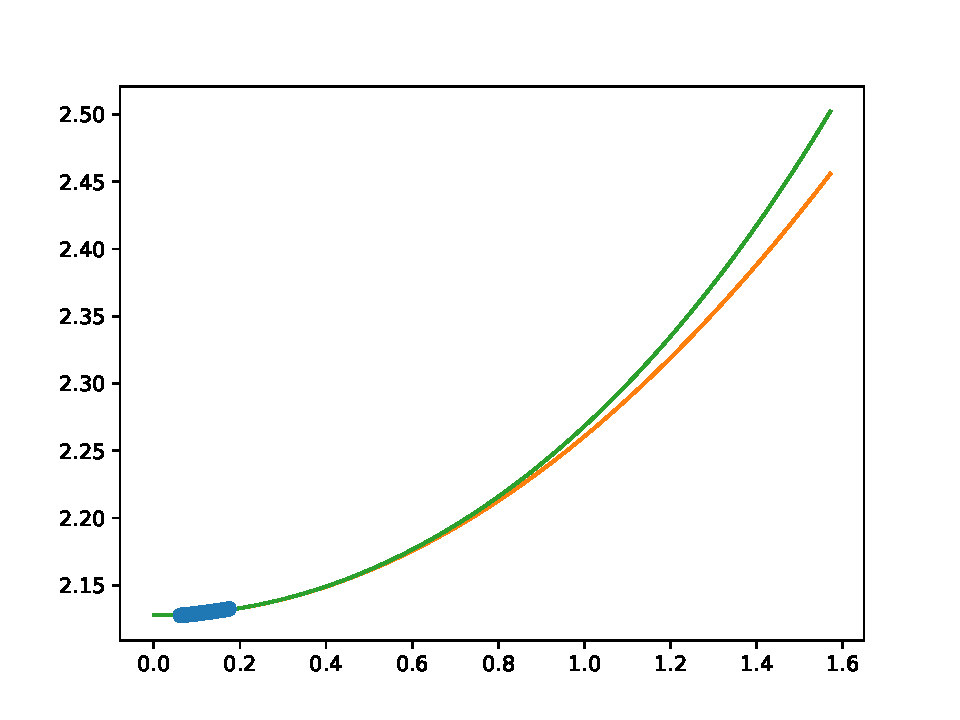
\includegraphics[scale=0.60]{Fit_piccola_ampiezza.pdf} \\
	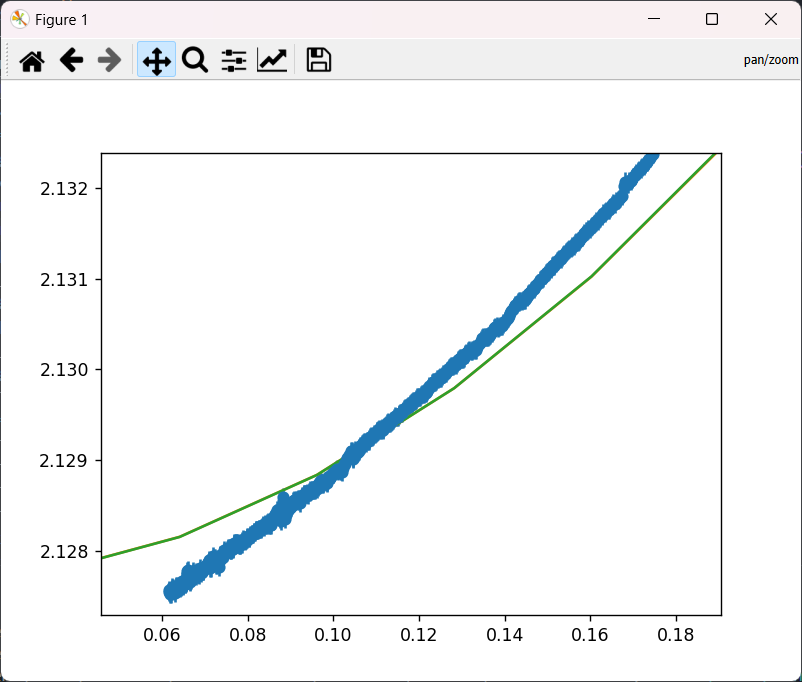
\includegraphics[scale=0.50]{zoom_piccole_ampiezze.png}
	\caption{Si osserva che i punti non si dispongono con un andamento parabolico come ci aspetteremmo: probabilmente il motivo deriva dal fatto che abbiamo fatto partire il pendolo da un'ampiezza troppo piccola per cui la dipendenza dell'angolo al secondo ordine era ancora trascurabile e ciò ha fatto sballare il fit}
\end{figure}

\noindent Come si può vedere dallo zoom nelle immagini qua sopra, le misurazioni non si dispongono con un assetto \emph{parabolico} sul modello teorico come ci aspettavamo: una spiegazione molto plausibile di ciò è dovuto al fatto che i valori che abbiamo misurato erano ancora troppi piccoli e la dipendenza dall'angolo del periodo era ancora trascurabile e, conseguentemente, il fit ne è uscito leggermente \emph{sballato}. Abbiamo a quel punto deciso di rieffettuare le misure facendo partire il pendolo da un'ampiezza più grande (circa $\ang{40}$) e abbiamo rieffettuato il grafico (riportato nella prossima pagina)

\begin{figure}[H]
	\centering
	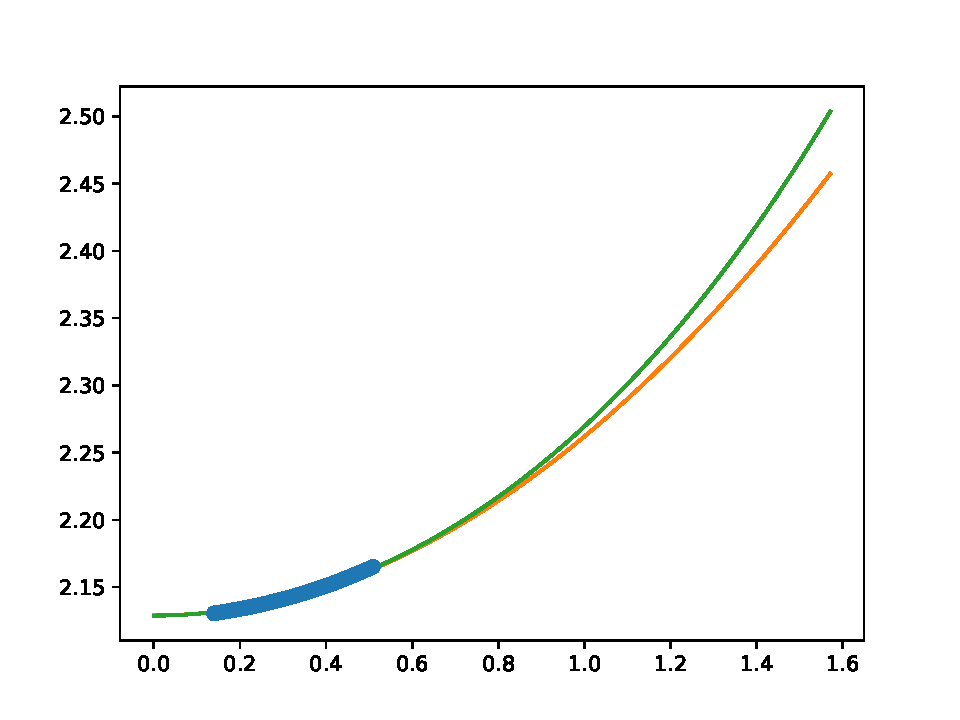
\includegraphics[scale=0.60]{Fit_ampiezza.pdf}
	\caption{Fit dei due modelli utilizzando le nuove misure: si osserva che questi nuovi dati, avendo fatto partire il pendolo da un'ampiezza maggiore, hanno un assetto più parabolico come ci si aspettava}
\end{figure}
Osserviamo il grafico dei residui di entrambi i due modelli teorici:

\begin{figure}[H]
\hspace{-0.025\textwidth}
\begin{minipage}{0.49\textwidth}
	\centering
	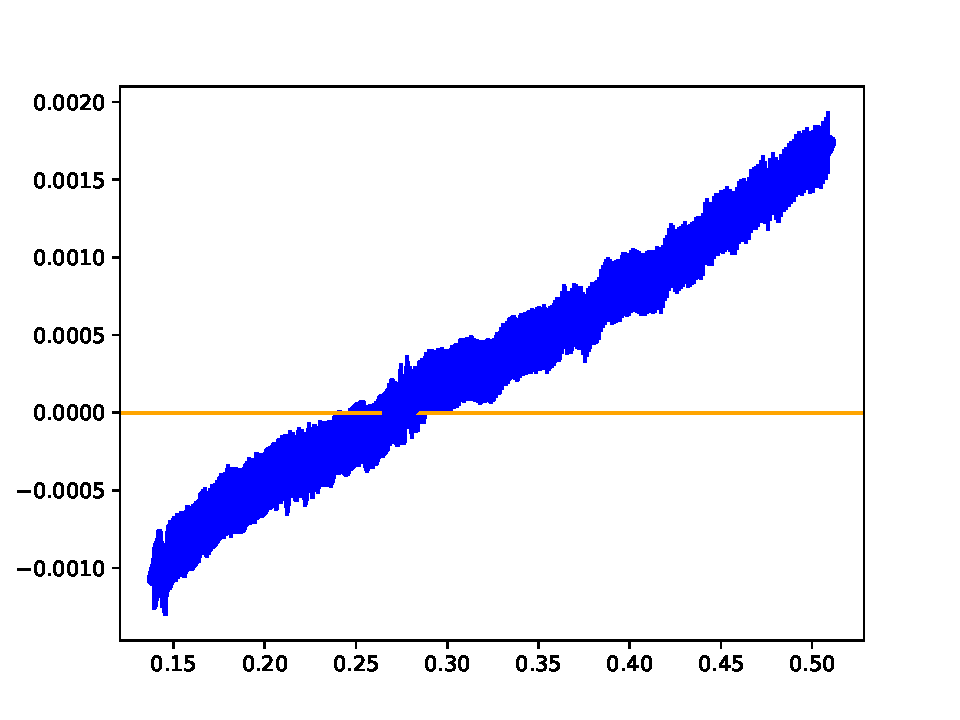
\includegraphics[scale=0.60]{Residui_taylor_2.pdf}
\end{minipage}
\hspace{0.005\textwidth}
\begin{minipage}{0.49\textwidth}
	\centering
	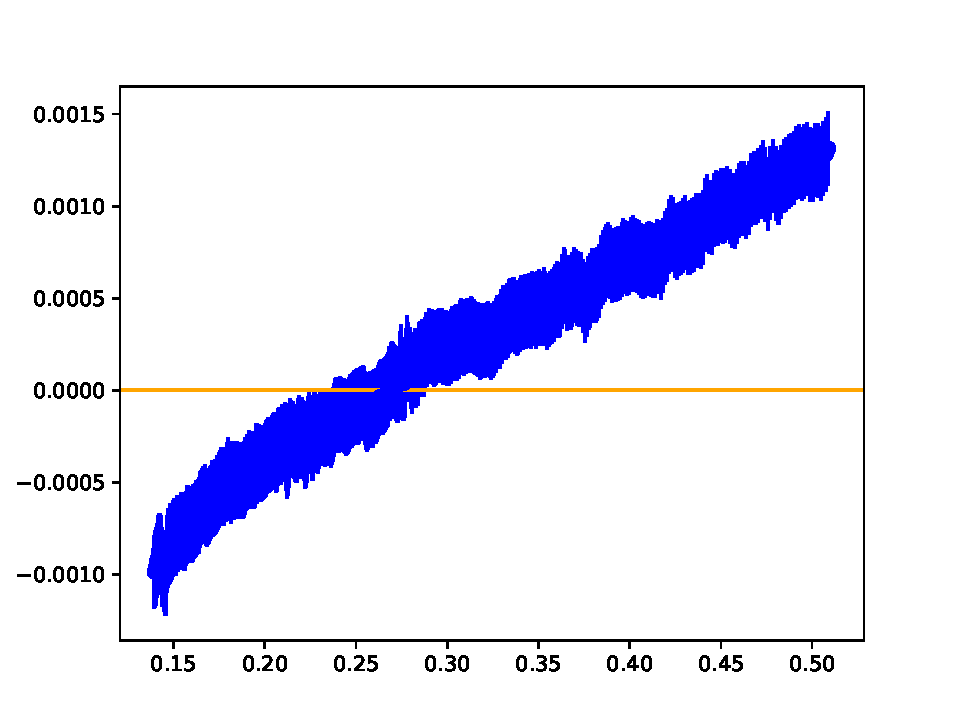
\includegraphics[scale=0.60]{Residui_taylor_4.pdf}
\end{minipage}	
	\caption{Residui dei due fit con i due modelli teorici. Il fatto che gli errori non sono compatibili con lo zero e la chiara asimmetria nelle permanenze che ci sono fra destra e sinistra è indice del fatto che le misure sono dominate dagli errori sistematici dovuti alle forze di attrito. Nonostante ciò, dall'analisi del $\chi^2$ si osserva che, come è lecito aspettarsi, l'espansione in serie di Taylor al quarto ordine possiede un $\chi^2$ minore siccome \emph{approssima} meglio la dipendenza fra il periodo in funzione dell'angolo $\theta$.}
\end{figure}

\noindent il fatto che gli errori non siano, per la maggior parte, compatibili con lo zero e l'asimmetria nelle permanenze sono un chiaro segnale che le incertezze di queste misure sono dominate da errori di natura non statistica: probabilmente, avendo fatto partire il pendolo da un'ampiezza maggiore, il pendolo possedeva una velocità maggiore e, dunque, l'attrito esercitato dall'aria che è proporzionale alla velocità ha influito maggiormente in queste misure: a testimonianza di ciò abbiamo rifatto studiato nuovamente, anche con questi dati, della dipendenza fra la velocità e il tempo e, in questo caso, la funzione \texttt{curve\_fit} stima dei parametri meno ragionevoli rispetto a quelli calcolati prima e, proprio come ci aspettavamo, il valore del $\chi^2$ è schizzato verso le stelle siccome sono aumentati gli effetti esercitati dalle forze di attrito che agiscono come errori sistematici: infatti, per quanto riguarda il parametro $v_0(0)$ noi ci aspettavamo un valore (misurato) di $v_0(0)$ pari a $(1.691 \pm 0.005) \, \si{\meter\per\second}$ e il fit stimava un valore di $\hat{v_0} = (1.624 \pm 0.002) \, \si{\meter\per\second}$, che non è assolutamente compatibile entro le barre di errore con il valore da noi misurato (siccome distano fra loro circa $12\sigma$). \\
Nonostante ciò dall'analisi del $\chi^2$ (che in questo caso ha poco senso siccome le misure non statisticamente indipendenti) possiamo osservare che l'espansione di Taylor al quarto ordine del periodo $T(\theta)$ è in migliore accordo, rispetto all'altro modello teorico, con le misure, siccome il $\chi^2 \approx 19934$ (che è un valore comunque molto alto ma giustificabile dalle dissipazioni dovute alle forze di attrito) mentre il $\chi^2$ dell'altro modello teorico è circa pari a $\chi^2 \approx 27635$.
Infine, abbiamo confrontato il valore $T_0$ stimato dal fit con quello misurato da noi: siccome si ha che
$$
	T_0 = 2 \pi \sqrt{\frac{l}{g}}
$$
gli abbiamo assegnato l'incertezza calcolata con la formula $\sigma_f(\theta_1, \theta_2, \cdots) = \sqrt{\left(\frac{\partial f}{\partial \theta_1} (\theta_1, \theta_2, \cdots) \sigma_{\theta_1} \right)^2 + \left(\frac{\partial f}{\partial \theta_2} (\theta_1, \theta_2, \cdots) \sigma_{\theta_2}\right)^2 + \cdots}$, pari a
$$
	\sigma_{T_0} = \frac{\pi \sqrt{\frac{l}{g}}}{l} \sigma_l
$$
dunque
\begin{equation}
	T_0 = (2.1513 \pm 0.0009) \, \si{\second}
\end{equation}
mentre i valori di $\hat{T_0}$ stimati rispettivamente dai due fit sono pari a:
\begin{align*}
	&T_0 = (2.12892 \pm 0.00006) \, \si{\second} \\
	&T_0 = (2.12883 \pm 0.00003) \, \si{\second} \\
\end{align*}
che già ad occhio si vede che non sono compatibili entro le barre di errore con il valore atteso: la motivazione è sempre quella espressa qua sopra, ovvero che le forze di attrito, facendo partire il pendolo da un'altezza maggiore, influivano maggiormente in questa presa dati.

\section{Conclusioni}
Sebbene l'esperimento non può considerarsi completamento un successo, siccome siamo riusciti a mostrare la legge che governa il \emph{decadimento} della velocità e non a verificare effettivamente la dipendenza fra il modello teorico previsto dalla teoria riguardo alla dipendenza fra il periodo $T$ e l'angolo $\theta_0$ a causa della presenza di errori sistematici dovuti alle forze di attrito, è stata comunque un'esperienza interessante per quanto riguarda l'effetto delle forze di attrito riguardo alle nostre misurazioni. Nonostante ciò sarebbe interessante ideare un esperimento per verificare la dipendenza fra il periodo e l'angolo in cui è possibile ridurre gli attriti con l'aria oppure ideare un modello teorico che contempla anche la presenza di forze di attrito.
\end{document}